\section{Daten filtern}

Aus Tabellen (Listen) können Daten nach bestimmten Kriterien gefiltert werden. Alle Zeilen, welche nicht dem Filterkriterium entsprechen werden dabei ausgeblendet.

Wenden Sie mehrere Filter an, so ist deren Wirkung kumulativ. Das bedeutet, dass der zweite Filter nur noch mit den Daten arbeitet, welche das erste Filter bereitstellt.

Generell ist zu beachten, dass in den Spalten immer nur ein Datentyp vorkommen darf, wie es auch relationale Datenbanken vorschreiben. Also sollen in einer Spalte z.B. immer nur numerische Werte oder Datumswerte vorkommen. Es soll also nicht sein, dass numerische mit nichtnumerischen Werten gemischt werden. Das Autofilter bietet nämlich vom Datentyp abhängige Filter automatisch an. Werden in einer Spalte gemischte Datentypen verwendet, dann wird das Filter für den am häufigsten vorkommenden Datentyp angeboten. 

Wird ein Filter auf eine Spalte angewendet,  für die bereits ein Filter existiert, wird der alte Filter automatisch gelöscht.


Grundsätzlich gibt es in Excel zwei verschiedene Filterarten
\begin{itemize}
	\smallitemize
	\item Autofilter
	\item Spezialfilter
\end{itemize}


\subsection{Autofilter}

\enlargethispage{1cm}
Bevor man das Autofilter einschaltet, sollte man eine Zelle im Datenbereich auswählen. Excel kann dann, wenn man die Überschriften anders als die Datenspalten formatiert hat, automatisch den kompletten Datenbereich auswählen. Danach wählt man \menu[,]{Daten, Sortieren und Filtern, Filter}.
	\begin{figure}[H]
		\centering
%		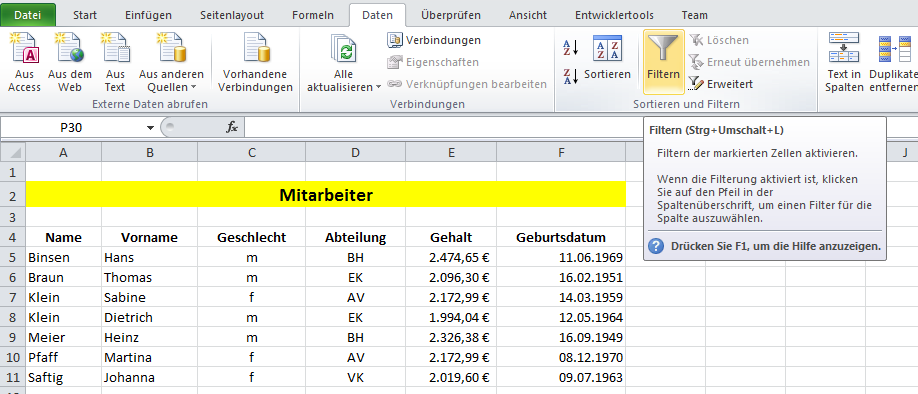
\includegraphics[width=12cm]{images/autofilter_raw.png}
			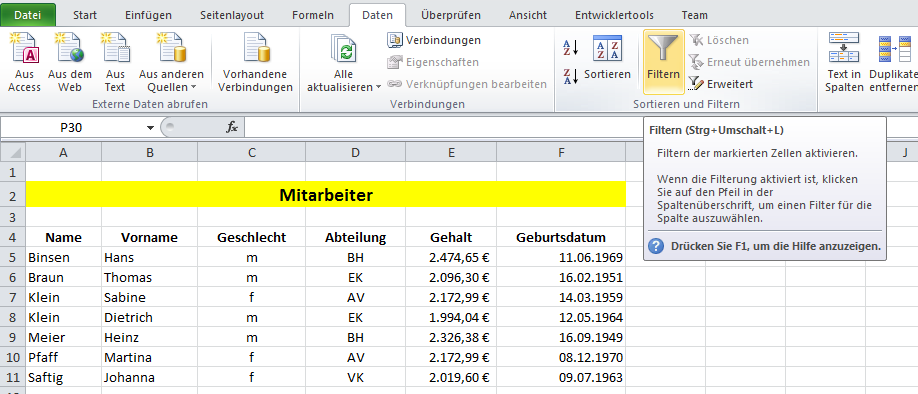
\includegraphics[scale=0.7]{images/autofilter_raw.png}
		\caption{Autofilter aus dem Menü auswählen}
		\label{fig:autofilterMenu}
	\end{figure}%
	\vspace{-1em}
Ist das Autofilter aktiviert, wird neben den Spaltenüberschriften ein kleines Dreieck für die Auswahl der Eingrenzungskriterien angezeigt und das Symbol im Ribbon wird aktiviert angezeigt.
	\begin{figure}[H]
		\centering
	%		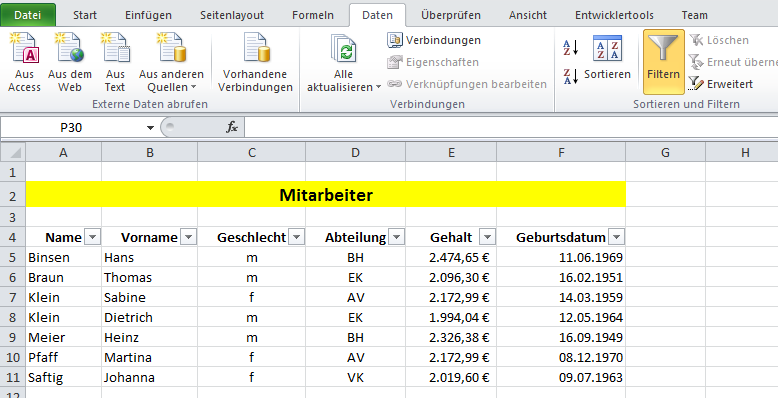
\includegraphics[width=12cm]{images/autofilter_on}
			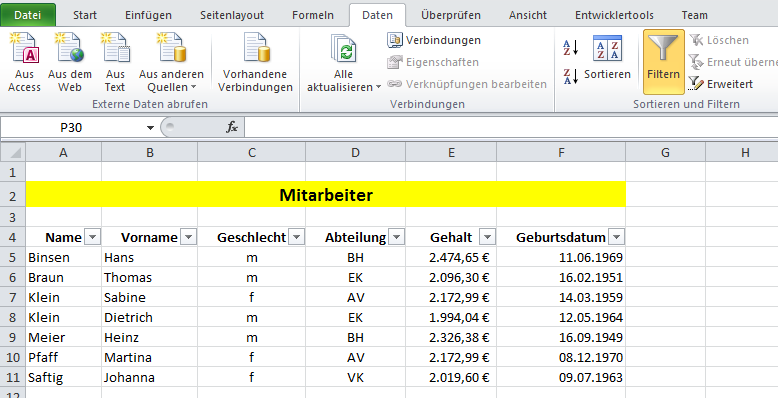
\includegraphics[scale=0.7]{images/autofilter_on}
		\caption{Eingeschaltetes Autofilter}
		\label{fig:autofilterOn}
	\end{figure}
Autofilter liefern schnell Ergebnisse, wenn es sich um einfache unkomplizierte Bedingungen handelt. Je nach Datentyp in einer Spalte zeigt das Autofilter unterschiedliche Optionen an.
	\begin{figure}[H]
		%\captionsetup[subfigure]{labelformat=empty}
   	\centering
		\subfloat[Autofilter bei Datumsspalten]{%
			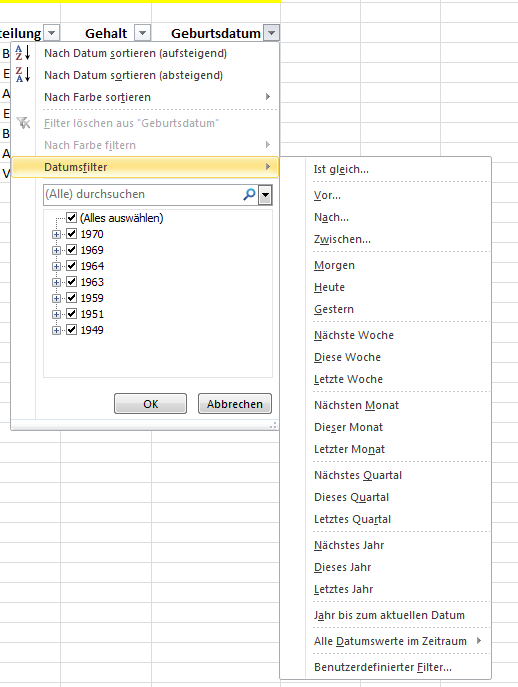
\includegraphics[width=5cm]{images/autofilter_datumsfilter}
			\label{fig:flowlayout1}
		}%
		\quad
		\subfloat[Autofilter bei Zahlenspalten]{%
			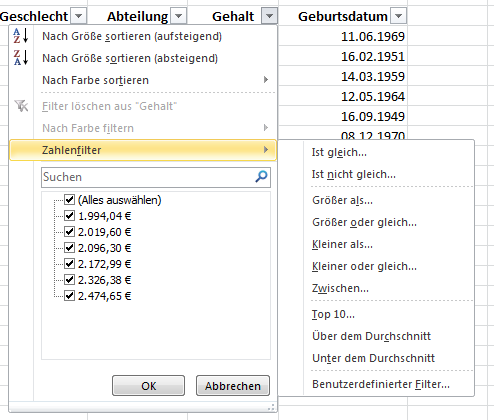
\includegraphics[width=5cm]{images/autofilter_zahlenfilter}
			\label{fig:flowlayout2}
		}%
		\quad
		\subfloat[Autofilter bei Textspalten]{%
			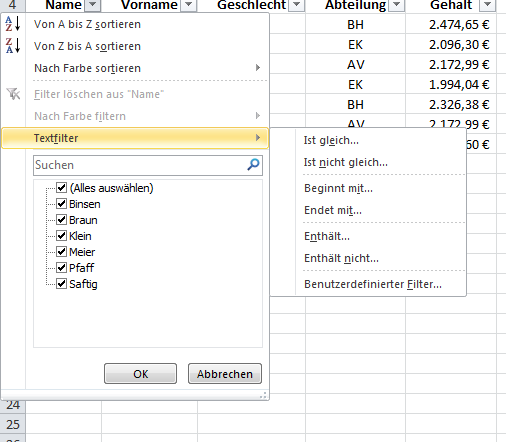
\includegraphics[width=5cm]{images/autofilter_textfilter}
			\label{fig:flowlayout3}
		}%
		\caption{Inhaltsabhängige Filtermöglichkeiten}
	\end{figure}
	
	
\subsection{\stmt{TEILERGEBNIS}}
	
Zeilen, welche nicht vom Filter betroffen sind, werden einfach ausgeblendet. Häufig ist man aber nicht an den einzelnen Datensätzen interessiert, sondern an aggregierten, d.h. zusammengefassten, Werten. Dies kann eine Summe, ein Durchschnitt oder Maximum sein. Die von Excel bekannten Funktionen nehmen allerdings keine Rücksicht auf ausgeblendete Zeilen, also sind sie für diese Aufgabenstellung nicht verwendbar. Um aggregierte Werte zu erhalten wird daher die \stmt{TEILERGEBNIS} Funktion verwendet.
$$ \text{\stmt{TEILERGEBNIS( \syntax{Funktion}; \syntax{Bezug}; \ldots; \syntax{[Bezug\_n]})}} $$%
%
Die \syntax{Funktion} gibt die Art der Aggregation an. Eine Auflistung der Aggregatsfunktionen mit ihren Funktionsnummern zeigt die \tabref{tab:teilergebnis}.
\begin{table}[H]
	\centering
		\begin{tabular}{@{}lcc@{}}
			\toprule  & \multicolumn{2}{c}{\textbf{Funktion}}\\
			 & \parbox[t]{5cm}{\centering berücksichtigt\\ausgeblendeten Zellen} & \parbox[t]{5cm}{ \centering ignoriert\\ausgeblendete Zellen}\\
			\midrule Mittelwert & 1 & 101\\
			Anzahl & 2 & 102 \\
			Anzahl2 & 3 & 103\\
			Max & 4 & 104 \\
			Min & 5 & 105 \\
			Produkt & 6 & 106 \\
			Stabw & 7 & 107 \\
			Stabwn & 8 & 108 \\
			Summe & 9 & 109 \\
			Varianz & 10 & 110 \\
			Varianzen & 11 & 111\\
		\end{tabular}
	\caption{Funktionsnummern der Aggregatfunktionen}
	\label{tab:teilergebnis}
\end{table}%
\vspace{-1em}
In der \figref{fig:teilergebnis} kann man sehen, wie sich ausgeblendete Zeilen auswirken. In der Tabelle ist die dritte Zeile ausgeblendet und die Funktion 109 liefert daher den um den Zellwert reduzierten Summenwert gegenüber der Funktion 9. In diesem Beispiel ist der Zellinhalt 3, die Summe also 12. \figref{fig:teilergebnisbeispiel} zeigt weiters die Gehaltssumme der Abteilung BH mit Hilfe des Autofilter und \stmt{TEILERGEBNIS}.
\enlargethispage{1cm}
	\begin{figure}[H]
		\centering
%			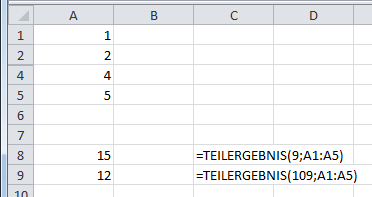
\includegraphics[width=8cm]{images/teilergebnis}
			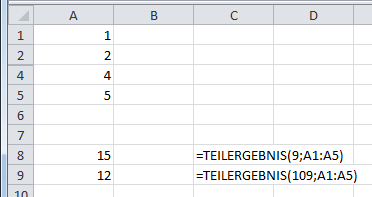
\includegraphics[scale=0.7]{images/teilergebnis}
		\caption{\stmt{TEILERGEBNIS} und ausgeblendete Zeilen}
		\label{fig:teilergebnis}
	\end{figure}%
%\pagebreak
\vspace{-1em}
%Für ein weiteres Beispiel wollen wir die Gehaltssumme der Abteilung BH mit Hilfe des Autofilter und \stmt{TEILERGEBNIS} ermitteln. 
	\begin{figure}[H]
		\centering
%			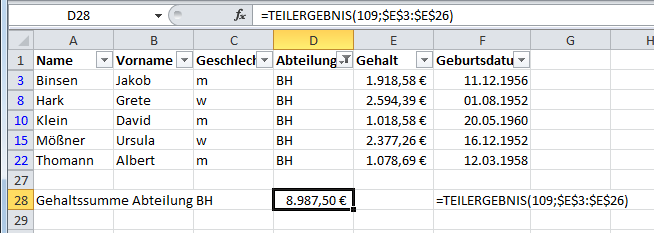
\includegraphics[width=8cm]{images/teilergebnis-beispiel}
			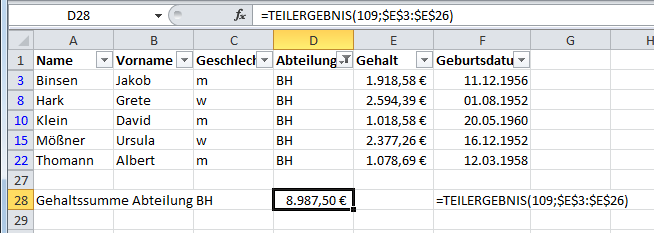
\includegraphics[scale=0.7]{images/teilergebnis-beispiel}
		\caption{Gehaltssumme der Abteilung BH mit \stmt{TEILERGEBNIS} }
		\label{fig:teilergebnisbeispiel}
	\end{figure}

\begin{lightbulbbox}
Es ist wichtig, dass alle Auswertungen, wie Berechnungen, Ergebnisse oder kopierte Ergebnisse von Spezialfiltern entweder oberhalb, unterhalb der Datengrundlage oder auf einem eigenen Tabellenblatt plaziert wird.

Es kann sonst passieren, dass durch das Filter diese Ergbnisse mit ausgeblendet werden und daher nicht mehr sichtbar sind!

\end{lightbulbbox}

%\pagebreak
\subsection{Spezialfilter}
\enlargethispage{1cm}
Mit dem Autofilter stoßen wir recht bald an die Grenzen der Übersichtlichkeit und Flexibilität. Das Spezialfilter ist ein mächtigeres Autofilter, bei dem die Filterkriterien explizit angeführt werden müssen.


	\begin{figure}[H]
		\centering
%			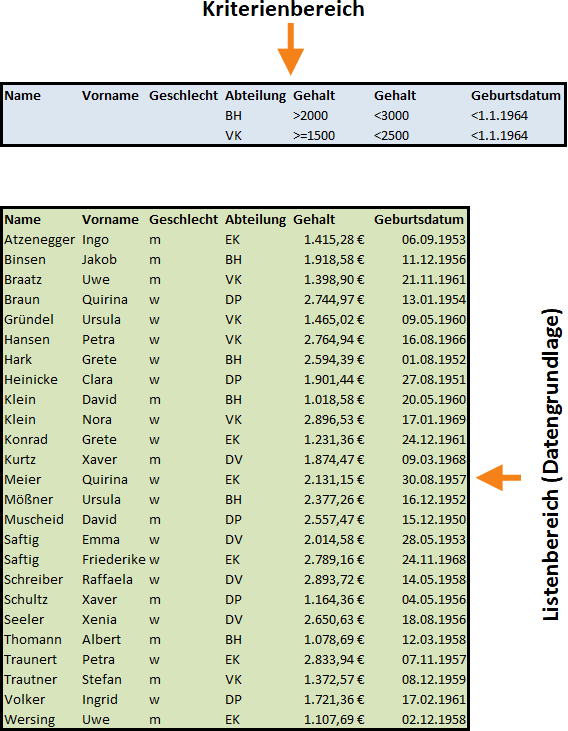
\includegraphics[width=8cm]{images/spezialfilter}
			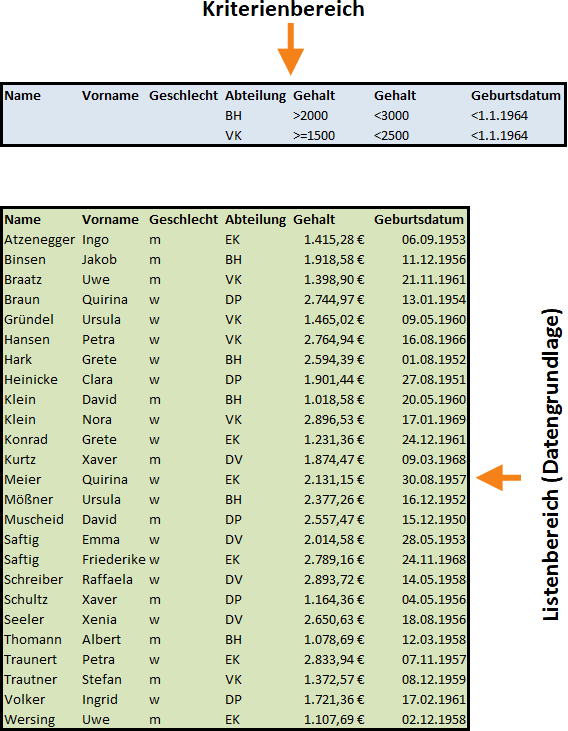
\includegraphics[scale=0.7]{images/spezialfilter}
		\caption{Spezialfilter mit Datenbereich und Kriterienbereich }
		\label{fig:spezialfilter}
	\end{figure}
	
	
\subsection{Spezialfilter Kriterienbereich}

Der Kriterienberreich des Spezialfilters wird benötigt, um Regeln zu erstellen, welche Datensätze gefiltert werden sollen

	\begin{figure}[H]
		\centering
%			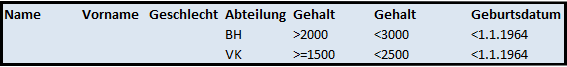
\includegraphics[width=12cm]{images/spezialfilter-kriterienbereich}
			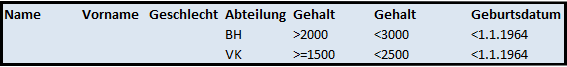
\includegraphics[scale=0.7]{images/spezialfilter-kriterienbereich}
		\caption{Spezialfilter Kriterienbereich }
		\label{fig:spezialfilterKriterienbereich}
	\end{figure}
	
Wie funktioniert nun das Filtern mit einem Spezialfilter? Vom Listenbereich kopiert man jene Überschriften, nach deren Wertinhalt gefiltert werden soll. Diese Überschriften kopiert man in einen Bereich oberhalb oder unterhalb des Listenbereiches. Soll in einer Spalte nach einem Bereich gefiltert werden, so muss die Überschrift zwei Mal abgebildet werden. Einmal für den Vergleich für die untere Grenze und ein Mal für die obere Grenze.
	
In oben gezeigtem Beispiel werden alle MitarbeiterInnen gefiltert, welche vor dem 1.1.1964 geboren wurden, in der Abteilung BH arbeiten und ein Gehalt von über 2.000 und unter 3.000 Euro erhalten. Des weiteren werden auch Datensätze von Mitarbeitenden angezeigt, welche vor dem 1.1.1964 geboren wurden, in der Abteilung VK arbeiten und ein Gehalt von mindestens 1.500 und unter 2.500 Euro verdienen.

\begin{lightbulbbox}
Merke:
\begin{itemize}
	\smallitemize
	\item Alle Spalten in einer Kriterienzeile sind \textit{UND} verknüpft
	\item Alle Zeilen des Kriterienbereiches sind \textit{ODER} verknüpft
\end{itemize}
\end{lightbulbbox}
%
\begin{lightbulbbox}
Es ist immer besser, wenn man die Spaltenüberschriften kopiert und nicht tippt, da sich Tippfehler einschleichen können. Tippfehler bewirken nämlich nicht, dass das Filtern nicht funktioniert, sondern man erhält ein berechnetes Feld, welches in \kapref{sec:berechneteFelder} noch näher erklärt wird.
\end{lightbulbbox}
	
\subsection{Spezialfilter Vergleichsoperationen}
	
\FloatBarrier
%\begin{figure*}[H]
\begin{table}[H]
	\centering
		\begin{tabular}{@{}p{4cm}p{2cm}@{}}
			\toprule \multicolumn{2}{c}{ \parbox[t]{6cm}{\centering \textbf{Vergleichsoperatoren für \\numerische- oder Datumswerte}}}\\
			\midrule ist gleich 20 &  $=20$\\
			größer $20$ & $>20$  \\
			größer gleich $20$ & $>=20$  \\
			kleiner $20$ & $<20$  \\
			kleiner gleich $20$ & $<=20$  \\
			ungleich $20$ & $<>20$\\
		\end{tabular}
	\caption{Numerische und Datumsvergleichsoperatoren}
\end{table}
%\end{figure*}
\vspace{-1em}
\FloatBarrier
%\begin{figure*}
\begin{table}[H]
	\centering
		\begin{tabular}{@{}p{9cm}p{6cm}@{}}
			\toprule \multicolumn{2}{c}{ \parbox[t]{9cm}{\centering \textbf{Vergleichsoperatoren für \\alphanumerische Werte}}}\\
			\midrule alle die mit "`Klein"' beginnen &  Klein\\
			alle die im Text "`Klein"' beinhalten & *Klein* \\
			 \parbox[t]{8cm}{alle Werte die mit A, B oder C beginnen\\ (D ist ausgeschlossen)}  & $<D$ \\
			 \parbox[t]{8cm}{alle Werte die mit X, Y oder Z beginnen\\ (Xx ist eingeschlossen)}  & $>X$ \\
			 beliebiges Zeichen an einer bestimmten Stelle & $?$ \\
			 kein, ein oder mehrere beliebige Zeichen & * \\
			 "`*"' als normales Zeichen & \~{}* \\
			 "`?"' als normales Zeichen & \~{}? \\
			 "`\~{}"' als normales Zeichen & \~{}\~{} \\
			 \parbox[t]{9cm}{Suchen nach exaktem Wert unter Berücksichtigung\\\quad der Groß- und Kleinschreibung} & =\stmt{IDENTISCH}(A5; "Klein"') \\
			 Suche nach leerer Zelle &  =\upquote{}\\
		\end{tabular}
	\caption{Alphanumerische Vergleichsoperatoren}
\end{table}
%\end{figure*}
\FloatBarrier

\subsection{Spezialfilter aktivieren}

Bevor man das Spezialfilter aktiviert, sollte man sich überlegen, wo die gefilterten Daten angezeigt werden sollen. Es gibt hierbei drei Möglichkeiten.
\begin{itemize}
	\smallitemize	
	\item An der gleichen Stelle wie die Datengrundlage anzeigen
	\item Am selben Tabellenblatt wie die Datengrundlage anzeichen, aber an anderer Stelle
	\item Auf einem anderen Tabellenblatt anzeigen
\end{itemize}

Die Vorgehensweise ist dabei identisch, es wird mit \menu[,]{Daten, Sortieren und Filtern, Erweitert} aufgerufen
	\begin{figure}[H]
		\centering
%			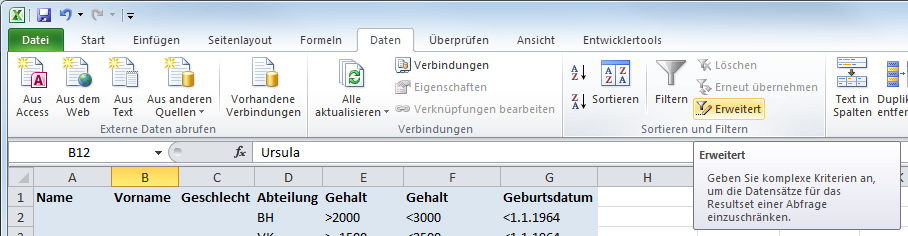
\includegraphics[width=12cm]{images/spezialfilter-menu}
			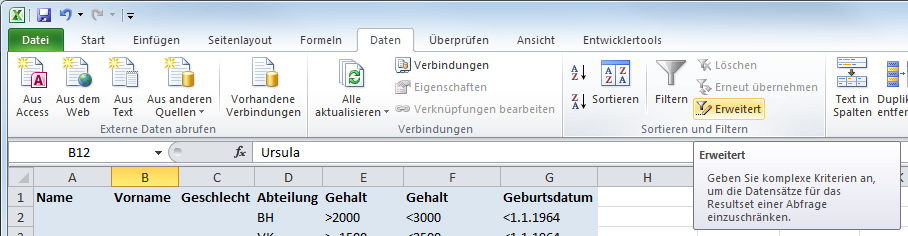
\includegraphics[scale=0.65]{images/spezialfilter-menu}
		\caption{Spezialfilter Menü}
		\label{fig:spezialfilterMenu}
	\end{figure}
	\vspace{-1em}
Danach wird in der Dialogbox entweder \textit{An gleicher Stelle filtern} gewählt, wenn die Daten im Listenbereich angezeigt werden sollen. Will man dagegen die Daten in einem anderen Bereich eines Arbeitsblattes oder in einem anderen Arbeitsblatt anzeigen, dann muss man \textit{An eine adere Stelle kopieren auswählen}
\enlargethispage{1cm}
	\begin{figure}[H]
		\centering
%			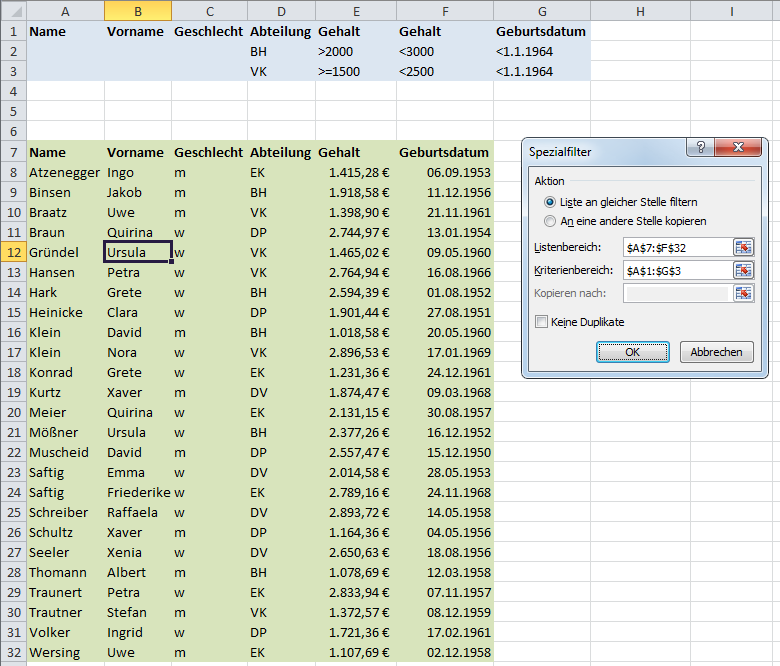
\includegraphics[width=12cm]{images/spezialfilter-dialogbox}
			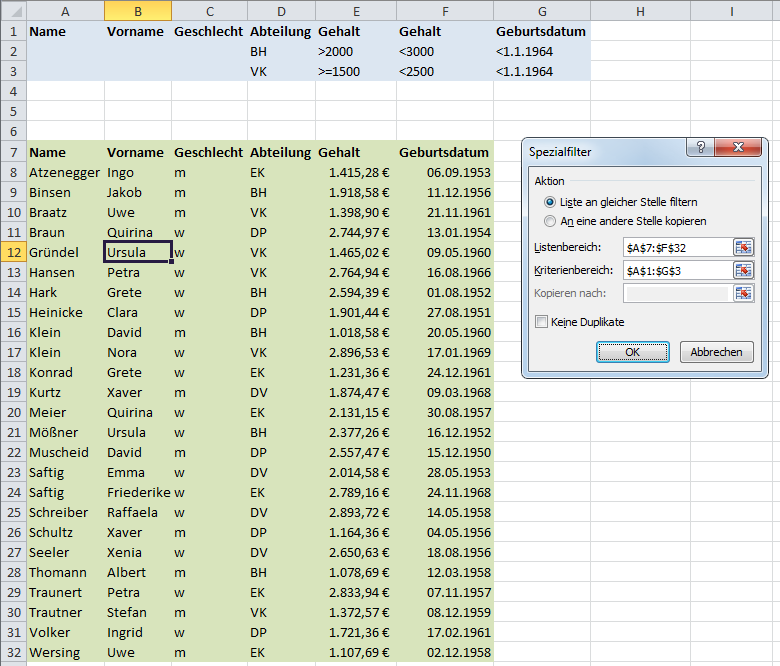
\includegraphics[scale=0.65]{images/spezialfilter-dialogbox}
		\caption{Spezialfilter aktivieren}
		\label{fig:spezialfilterAktivieren}
	\end{figure}

\begin{lightbulbbox}
Will man die gefilterten Daten am gleich Datenblatt haben, so empfielt es sich, dass man vor dem Aufrufen des Spezialfilters den Cursor innerhalb des Datenbereiches setzt, da dieser dann automatisch von Excel erkannt und ausgewählt wird.
\end{lightbulbbox}
%\pagebreak
\begin{lightbulbbox}
Eine besondere Falle liefert Excel, wenn das Ergebnis auf ein anderes Tabellenblatt kopiert werden soll. Man muss \textit{immer} zwingend von dem Tabellenblatt ausgehen, auf dem die gefilterten Daten angezeigt werden. Macht man dies nicht, so liefert Excel die Fehlermeldung%
	\begin{figure}[H]
	%\vspace{2em}
		\centering
%			
\includegraphics[width=8cm]{images/spezialfilter-fehler2010}
			
\includegraphics[scale=0.7]{images/spezialfilter-fehler2010}
		\caption{Spezialfilter Fehlermeldung}
		\label{fig:spezialfilterFehlermeldung}
	\end{figure}
\end{lightbulbbox}


\subsection{Spezialfilter mit berechneten Feldern}
\label{sec:berechneteFelder}

Eine Besonderheit im Kriterienbereich sind berechnete Felder. Im Gegensatz zu normalen Kriterien wird hier nicht direkt eine Spalte der Datengrundlage mit einem Wert verglichen, sondern der zu vergleichende Wert wird über eine Formel bestimmt. Berechnete Felder kommen zum Einsatz, wenn an der Datengrundlage nichts geändert werden darf oder kann.

Nehmen wir als Beispiel, dass wr alle MitarbeiterInnen der Abteilung BH herausfinden wollen, welche ein Jahreseinkommen von über 30.000\texteuro\ haben.  Das Jahreseinkommen ist das 14-fache des Monatsgehaltes plus der Zulage. 

Bei berechneten Feldern sind folgende Dinge zu beachten
\begin{itemize}
	\smallitemize
	\item Die Überschrift im Kriterienbereich darf  \textit{niemals} mit einer der Überschriften der Datengrundlage übereinstimmen. Der Grund liegt darin, dass es sich hier um eine "`künstliche"' Spalte handelt.
	\item Berechnete Felder beginnen immer mit $=$, da es sich um eine Formel handelt
	\item Die Formel in berechneten Feldern muss immer \stmt{WAHR} oder \stmt{FALSCH} ergeben
	\item Wenn bei der Berechnung Werte der Datengrundlage herangezogen werden, muss \textit{immer} der Wert aus der \textit{ersten} Zeile der Datengrundlage genommen werden.
\end{itemize}
\enlargethispage{2cm}
Wie wird das nun in der zu lösenden Aufgabe umgesetzt?
	\begin{figure}[H]
		\centering
%			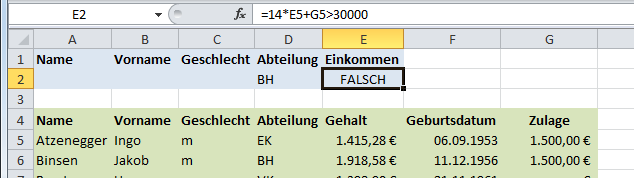
\includegraphics[width=10cm]{images/spezialfilter-berechnet1}
			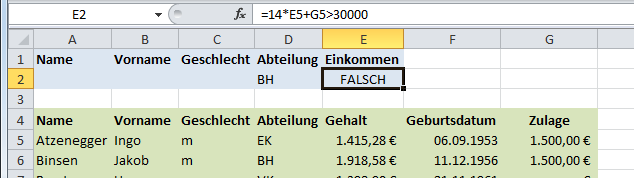
\includegraphics[scale=0.7]{images/spezialfilter-berechnet1}
		\caption{Spezialfilter mit berechnetem Feld}
		\label{fig:spezialfilterBerechnetesFeld}
	\end{figure}
	
	
	
Die Formel für die Berechnung lautet $14*Gehalt+Zulage$. Mit dieser Formel soll jede Zeile des Listenbereichs verglichen werden. Ist das Ergebnis größer als 30.000, dann soll diese Zeile im Ergebnis aufscheinen. Die erste Zeile des Listenbereiches ist die Zeile 5, also muss diese für den Vergleich herangezogen werden. Das Kriterium lautet daher
\begin{equation}
	\text{\stmt{= 14 * E5 + G5 > 30000}}
\end{equation}
wie auch in der Abbildung ersichtlich ist.


\section{Datenbankfunktionen}

Datenbankfunktionen ermöglichen eine aggregierte Auswertung großer Listen mit komplexen Filterkriterien, die identisch aufgebaut sind, wie jene des Spezialfilter Kriterienbereiches. Deswegen sie sehr oft in Zusammenhang mit dem Spezialfilter vwerwendet, da sie neben dem reinen Filtern von Datensätzen auch wichtige Informationen wie Maximum Minimum oder Summe eines gefilterten Datenbereiches liefern. Im Prinzip kann da auch die bereits bekannte \stmt{TEILERGEBNIS} Funktion, welche aber den Nachteil hat, dass bei geänderten Bedingungen \textit{keine} Neuberechnung stattfindet.

Die Datenbankfunktionen sind

\begin{multicols}{2}
	\begin{itemize}
	\smallitemize
    	\item \stmt{DBANZAHL}
	    \item \stmt{DBANZAHL2}
    	\item \stmt{DBMAX}
    	\item \stmt{DBMIN}
	    \item \stmt{DBPRODUKT}
    	\item \stmt{DBMITTELWERT}
    	\item \stmt{DBSTDABWN}
	\end{itemize}
\end{multicols}

Die Anzahl und der Aufbau der Parameter der Datenbankfunktionen sind bei alles oben genannten gleich, daher folgt hier die Beschreibung anhand von \stmt{DBSUMME}.
$$ \text{\stmt{DBSUMME( \syntax{Datenbank}; \syntax{Datenbankfeld}; \syntax{Suchkriterien})}} $$
\pagebreak
\begin{description}[labelindent=0cm, leftmargin=3.5cm, font=\mdseries, labelwidth=3cm,style=nextline]
\smallitemize
\item[\syntax{Datenbank}]Ist die Datengrundlage \textit{inklusive} der Überschriften
\item[\syntax{Datenbankfeld}] Ist die Spalte an der die Datenbankfunktion durchgeführt werden soll. Wichtig ist hier, dass die Überschrift der Spalte ausgewählt wird.
\item[\syntax{Suchkriterien}] Diese bestimmen, genauso wie beim Kriterienbereich des Spezialfilters, welche Datensätze für die Aggregatfunktion herangezogen werden sollen. Wie auch beim Spezialfilter werden im Kriterienbereich Spalten \stmt{UND} verknüpft und Zeilen \stmt{ODER} verknüpft.
\end{description}
%
%\pagebreak
Als Beispiel will ein Controller folgende Dinge in einem Unternehmen wissen
\begin{itemize}
	\smallitemize
	\item wie viele Mitarbeiter arbeiten in der Abteilung VK,
	\item wie viele Mitarbeiter sind davon über 50 Jahre alt,
	\item die Gehaltssumme der Abteilung VK
\end{itemize}

	\begin{figure}[H]
		\centering
%			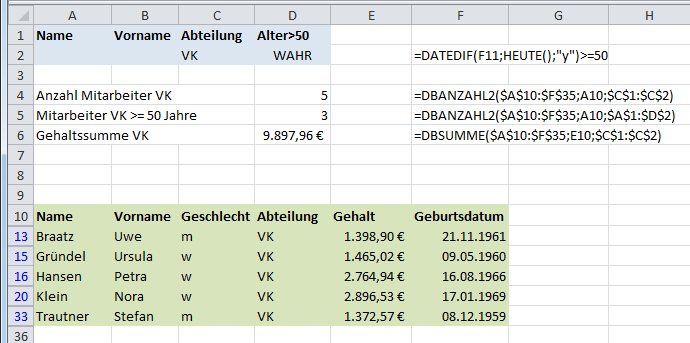
\includegraphics[width=10cm]{images/datenbankfunktion}
			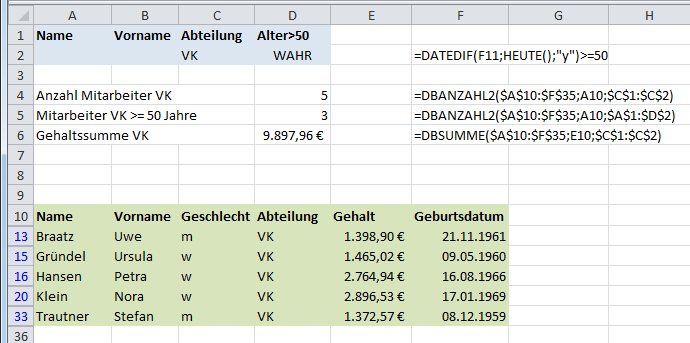
\includegraphics[scale=0.7]{images/datenbankfunktion}
		\caption{Datenbankfunktionen}
		\label{fig:datenbankfunktionen}
	\end{figure}

Will der Controller nun statt der Abteilung VK jetzt die Abteilung EK wissen, braucht er nur in der Zelle \xlc{C2} den Wert \upquote{VK} auf \upquote{EK} ändern und erhält sofort das Ergebnis.
